
\usetikzlibrary{arrows.meta,calc,patterns,shapes}
\providecommand{\computer}{%
    
\includegraphics[width=1cm]{../common/Noun_project_216.pdf}
}
\providecommand{\switch}{%
    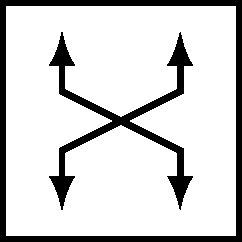
\includegraphics[width=0.9cm]{../common/fig-switch.pdf}
}
\providecommand{\bigswitch}{%
    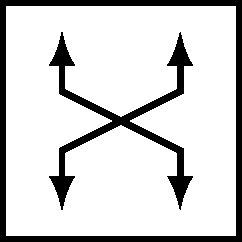
\includegraphics[width=1.4cm]{../common/fig-switch.pdf}
}
\providecommand{\router}{%
    
\includegraphics[width=0.9cm]{../common/fig-router.pdf}
}


\begin{frame}{connecting two networks}
\begin{tikzpicture}
\tikzset{
    connect/.style={draw,very thick,Latex-Latex},
    computer/.style={inner sep=0mm,outer sep=0mm,execute at begin node={\computer}},
    switch/.style={inner sep=0mm,outer sep=0mm,execute at begin node={\switch}},
    big switch/.style={inner sep=0mm,outer sep=0mm,execute at begin node={\bigswitch}},
    router/.style={inner sep=0mm,outer sep=0mm,execute at begin node={\router},circle},
    packet/.style={minimum width=.4cm,minimum height=0.2cm,inner sep=0mm,outer sep=0mm,draw},
    packet lg/.style={minimum width=.6cm,minimum height=0.2cm,inner sep=0mm,outer sep=0mm,draw},
    c1c2/.style={fill=violet!40,draw=black,thin,alt=<2>{thick,draw=red}},
}
\begin{scope}
    \node[cloud,aspect=2] (site A) at (0, 0) {company site A};
    \node[cloud,aspect=2] (site B) at (6, 0) {company site B};
    \node[cloud,aspect=2,minimum height=3cm] (internet) at (3, 6)  {
        internet
    };
    \node[router,anchor=south] (A route) at ([yshift=.5cm]site A.north) {};
    \node[router,anchor=south] (B route) at ([yshift=.5cm]site B.north) {};
    \foreach \x/\y in {site A/A route,site B/B route} {
        \draw[connect] (\x) -- (\y);
    }
    \draw[dotted,line width=1mm,dotted] 
        (A route.north) -- ([yshift=-1cm,xshift=-1cm]internet.center)
            -- ([yshift=-1cm,xshift=1cm]internet.center) -- (B route.north);
\end{scope}
\node at (3, 7) { reality };
\node at (3, 7) { illusion };
\draw[ultra thick] (6.5, -1) -- ++ (0, 7);
\begin{scope}[xshift=7cm,name prefix=alt-]
    \node[cloud,aspect=2] (site A) at (0, 0) {company site A};
    \node[cloud,aspect=2] (site B) at (6, 0) {company site B};
    \node[cloud,aspect=2,minimum height=3cm] (internet) at (3, 6)  {
        internet
    };
    \node[router,anchor=south] (A route) at ([yshift=.5cm]site A.north) {};
    \node[router,anchor=south] (B route) at ([yshift=.5cm]site B.north) {};
    \foreach \x/\y in {site A/A route,site B/B route} {
        \draw[connect] (\x) -- (\y);
    }
    \draw[connect] (A route) -- (B route);
\end{scope}
\end{tikzpicture}
\end{frame}

